\documentclass[xcolor=table]{beamer}

\usepackage{graphicx, natbib, tikz, subcaption}
\usepackage[export]{adjustbox}

\usepackage{xcolor}


\usetikzlibrary{decorations.pathreplacing,arrows}

\title{Binary Dependent Variable}
\subtitle{GV 903 Week 16}
\date{January 18, 2023}
\author{Winnie Xia}


\usetheme[progressbar=frametitle]{metropolis}
%\usecolortheme{seahorse}

\begin{document}
\beamertemplatenavigationsymbolsempty

\frame{
\titlepage
}

\frame{
\frametitle{Binary Data} 
\begin{itemize}
	\item A variable is binary if it only has two values, 0 or 1 ("No" or "Yes", etc.)
	\begin{itemize}
	\item Did you vote or not?
	\item Did a country adopt this new policy or not?
	\item Did the war or protest end or not?
	\end{itemize}
\end{itemize}
}

\frame{
\frametitle{Why not linear model}
\begin{itemize}
	\item A typical OLS equation looks like:
	$$ Y = \beta_0 + \beta_1X + \varepsilon $$
	and assumes that the error term, $\varepsilon$, is normal. \pause
	\item Running OLS with a binary dependent variable is called \textbf{linear probability model}. \pause
	\item The interpretation is the exact same as regular OLS. The only difference is that our interpretation of the dependent variable is now in probability terms. \pause
	\item So we say, \textbf{a one-unit increase in $X$ is associated with a three percentage point increase in the probability}. 
	
\end{itemize}
}

\frame{
\frametitle{Why not linear model}
\begin{itemize}
	\item We will get prediction outside the interval between 0 and 1. \pause
	\item Violate the homoscedasticity assumption of OLS. \pause
	\item By using OLS estimator, we assume linear trend in probabilities.  
\end{itemize}
}

\frame{
\frametitle{Generalized Linear Model}
\begin{itemize}	
	\item A GLM equation looks like:
	 $$ E(Y | X) = F(\beta_0 + \beta_1X) $$
	\item Key difference: 
	\begin{itemize}
	\item \textbf{estimated by maximum likelihood}, rather than OLS.
	\item \textbf{binomial distribution for binary data}, rather than normal distribution.
	\item In R, \textbf{glm()}, rather than lm().
	\end{itemize}
\end{itemize}
}

\frame{
\frametitle{Probit vs. Logit}
\begin{itemize}
	\item Logit model is a form of a statistical model that is used to predict the probability of an event occurring
	\item Probit model is similar to logit model, but it determines the likelihood that an item or event will fall into one of a range of categories by estimating the probability that observation with specific features will belong to a particular category.
	\item So dependent variable for probit model can only take on \textbf{one of the two values, such as yes or no, true or false}.
\end{itemize}
}

\frame{
\frametitle{Probit vs. Logit}
Logit models are used to \textbf{model logistic distribution} while probit models are used to model the \textbf{cumulative standard normal distribution}.
\begin{figure}
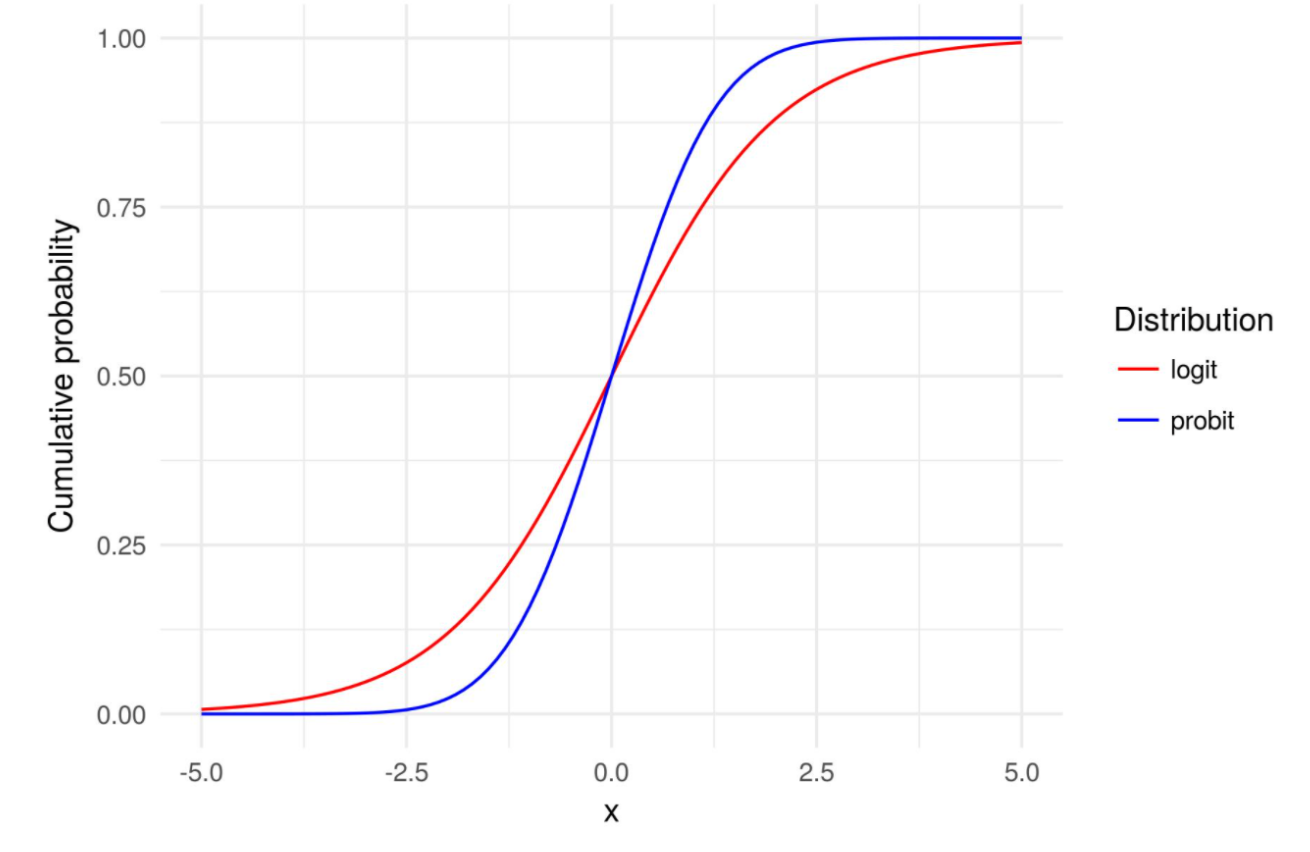
\includegraphics[width = 7 cm]{probit_logit.png}
\end{figure}
}


\frame{
\frametitle{Interpretation}
\begin{itemize}
	\item Coefficients are log odd-ratios. \pause
	\item From the coefficients themselves we can get direction (positive/negative) and significance, but not \textbf{the size of effect}. \pause
	\item So we convert them into odds-ratio by exponentiating: 	
	expo(coef(mode))
\end{itemize}
}

\frame{
\frametitle{How to interpret odds ratio}
\begin{itemize}
	\item 1 is the reference point. \pause
	\item Odds ratio above 1 increased occurrence of an event.  \pause
	\item Odds ratio below 1 decreased occurrence of an event. 
\end{itemize}
}

\frame{
\frametitle{Predicted Probability/ Marginal effect}
\begin{itemize}
	\item To interpret the effects more clearly, we need to calculate the predicted probability. \pause
	\begin{itemize}
	\item predict(model, newdata, type="response")
	\item And we write, \textbf{the predicted probability for the occurrence of an event is ***}.
\end{itemize}	
\end{itemize}

}

\end{document}